\newpage 

\section*{Appendix}

  
\section{Ablation Study}

We conducted experiments to recreate the MNIST Ablation Study. For this study, the pre-trained model provided by the authors was used. We observed a similar trend to the authors. An increase in the number of counterfactual images used in training resulted in higher training accuracies. However, our values differed significantly from those in the report, as seen in Fig. \ref{fig:mnist-ablation-ours} and Fig.  \ref{fig:mnist-ablation-theirs} . In particular, we observed higher accuracies for each dataset, especially when only $10^4$ counterfactuals were used in training. This difference may be explained by differences between the pre-trained models provided by the authors and the models that were used to generate the plots.

\begin{figure}[ht!]
    \centering
    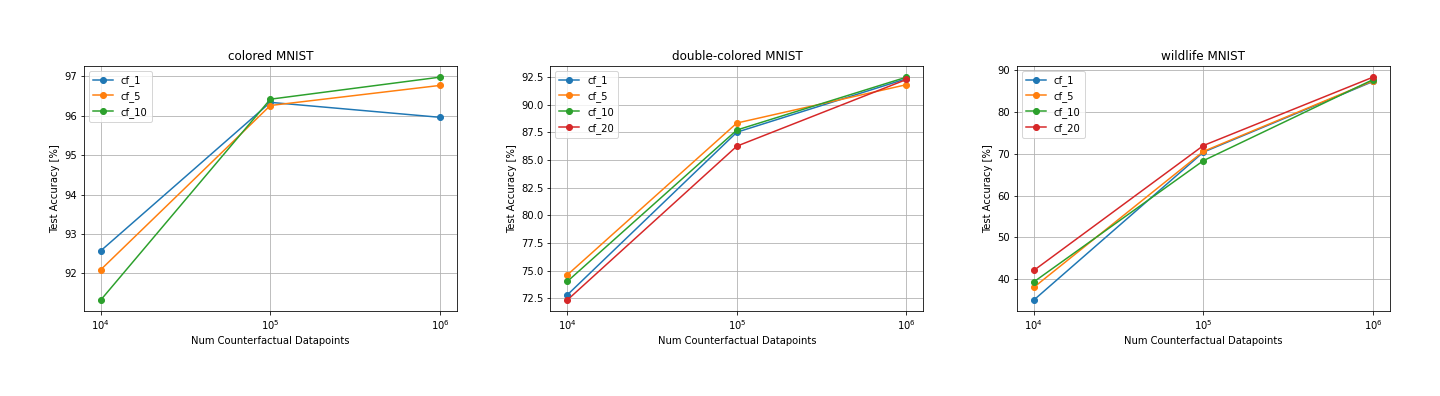
\includegraphics[width = 15cm]{../openreview/images/ablation.png}
    \caption{Recreated MNIST Ablation Study}
    \label{fig:mnist-ablation-ours}
\end{figure}


\begin{figure}[h!]
     \centering
     \begin{subfigure}{0.3\linewidth}
         \centering
         \includegraphics[width=\textwidth]{../openreview/images/image-085.png}
     \end{subfigure}
     \begin{subfigure}{0.3\linewidth}
         \centering
         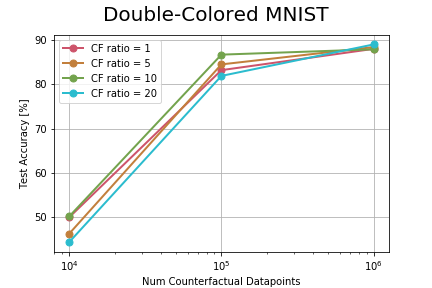
\includegraphics[width=\textwidth]{../openreview/images/image-087.png}
     \end{subfigure}
     \begin{subfigure}{0.3\linewidth}
         \centering
         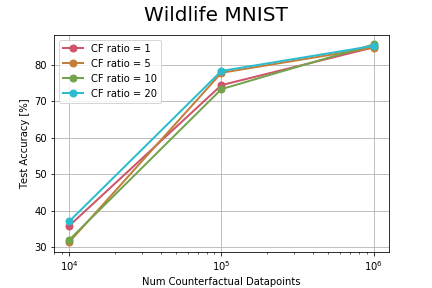
\includegraphics[width=\textwidth]{../openreview/images/image-089.png}
     \end{subfigure}
        \caption{Original MNIST Ablation Study from CGN\cite{sauer2021counterfactual}}
    \label{fig:mnist-ablation-theirs}
\end{figure}


% pending: first compare all tables, ablation studies of paper vs ours. Then start with extra results such as hyper parameter search, ssim, data augmentation etc. For every table lets state experimental details and adding visual outputs of masks, bg, fg and xgen. Can we add latent space tsne pots, or pca to visualise the plots. add graph logging since that can help as a code contribution, and also can generate graphs that can be added to paper. \cite{sauer2021counterfactual}

\section{Training time for Generative Model}

The following table shows the training time for each generative network against the dataset that was used.

Note: The ImageNet based CGN depends only on the BigGAN-256 backbone and U2-net to train. The MNIST based CGN architecture however, trains using the dataset without any pre-trained weight as backbone.
ImageNet counterfactual generation was going to run for 1.2 million iterations(0.5s/iteration), which was not computationally feasible with our resources.

\begin{table}[h]
\centering
\begin{tabular}{|l|l|l|}
\toprule
{} & Training time\\
{} & (in hours) \\
Dataset & \\
\midrule
Colored MNIST & \approx0.6\\
Double-colored MNIST & \approx0.6\\
Wildlife MNIST       & \approx3.5\\
Imagenet & \approx$167\\
\end{tabular}
\caption{Training time for CGN for different datasets}
\label{table:training_time_cgn}
\end{table}


\section{Counterfactual Images}
The following images using the pre-trained CGN model that was provided with the codebase. Minor deviations were observed with the image given in the paper to the result we obtained. 
\begin{figure}[ht!]
\centering
    \includegraphics[width=0.9\textwidth,height=0.3\textwidth]{../openreview/counterfactuals/xgen_1.pdf}
    \caption{Grid of Counterfactual Images from the Pre-trained CGN \cite{sauer2021counterfactual} as given in the original paper. The CGN is trained with biggan-256 as the backbone and Pre-trained U2-net for mask generation.  
    }
    \label{fig:original_counterfactuals}
\end{figure}

\begin{figure}[ht!]
\centering 
    \includegraphics[width=0.9\textwidth,height=0.3\textwidth]{../openreview/counterfactuals/xgen_2.pdf}
    \caption{Grid of Counterfactual Images from same class that have poorer x{gen}.
    All classes are picked at random and the counterfactual analysed for 'realism'}
    \label{fig:poor_counterfactuals}
\end{figure}

\begin{figure}[h!]
    \centering
    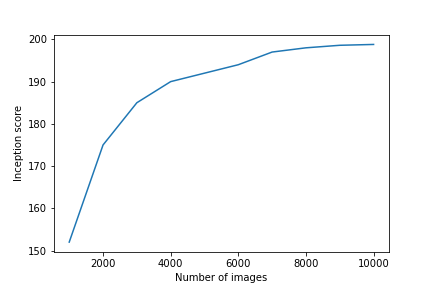
\includegraphics[width=10cm]{../openreview/images/inception.png}
    \caption{Inception score (10 splits) of images generated by the pre-trained CGN}
    \label{fig:inception}
\end{figure}

\newpage
\section{SSIM Loss function}
SSIM \cite{wang2004image} helps preserve the structural properties between the two images by using luminance, contrast and structural information. Additionally, SSIM \cite{wang2004image} leads to generating better structured masks using the 'm' that helps to localize the digits in a better way in the final output $x_{gen}$.

SSIM \cite{wang2004image} is defined using the three aspects of similarities, luminance $\big(l(\mathf{x}, x_{gen})\big)$, contrast $\big(c(\mathf{x}, x_{gen})\big)$ and structure $\big(s(\mathf{x}, x_{gen})\big)$ that are measured for a pair of images $\{\mathf{x}, x_{gen}\}$ as follows:
Given two images ground truth $\mathf{x}$ and generated image $x_{gen}$, the SSIM \cite{wang2004image} loss is defined \cite{pandey2020unsupervised} as follows:
\begin{equation}
\mathcal{L}_{ssim}(\alpha) = 1-\mathbf{E}_\mathf{x}\left[l(\alpha).cs(\alpha)\right]
\label{ssim_loss}
\end{equation}
\begin{equation}
l(\mathf{x}, x_{gen}) = \frac{2\mu_\mathf{x}\mu_{x_{gen}}+C_1}{\mu_\mathf{x}^2+ \mu_{x_{gen}}^2 + C_1}
\end{equation}
\begin{equation}
c(\mathf{x}, x_{gen}) = \frac{2\sigma_{\mathf{x}}\sigma_{x_{gen}}+C_2}{{\sigma_\mathf{x}}^2+ {\sigma_{x_{gen}}}^2 + C_2}
\end{equation}
\begin{equation}
s(\mathf{x}, x_{gen}) = \frac{\sigma_{\mathf{x}{x_{gen}}}+C_3}{\sigma_{\mathf{x}}\sigma_{x_{gen}} + C_3}
\end{equation}
where $\mu$'s denote sample means and $\sigma$'s denote variances. $C_1, C_2$ and $C_3$ are constants. With these, SSIM and the corresponding loss function $\mathcal{L}_{ssim}$, for a pair of images $\{\mathf{x}, x_{gen}\}$ are defined as: 
\begin{equation}
\text{SSIM}(\mathf{x}, x_{gen}) = l(\mathf{x}, x_{gen})^{\alpha} \cdot c(\mathf{x}, x_{gen})^{\beta} \cdot s(\mathf{x}, x_{gen})^{\gamma}  
\end{equation}
where $\alpha>0$, $\beta>0$ and $\gamma>0$ are parameters used to adjust the relative importance of the three components.
\begin{equation}
\mathcal{L}_{ssim}(\mathf{x}, x_{gen}) = 1 - \text{SSIM}(\mathf{x}, x_{gen})
\end{equation}

\subsubsection{Additional Result 2 - Exploring the biased behaviour of CGN\cite{sauer2021counterfactual} with the datasets}

% @Sameer -- proposed change to the color jitter para:

To investigate the robustness of the CGN architecture \cite{sauer2021counterfactual} to varied color augmentations, we applied color jitter to augment the training data. We found that applying a color jitter decreased classification accuracy by 10\% on double-colored MNIST and 50\% on wildlife MNIST.


% To investigate the dependence of CGN \cite{sauer2021counterfactual} in scenarios where the source data can have diverse colored image backgrounds and diverse colored digits, we add color jitter as an augmentation to the training data loader of the CGN function. 
Amongst all widely known augmentations we make use of color jitter since from \cite{chen2020simple}, \cite{he2020momentum} it is evident that color jitter, sobel flter augmentations are imperative to learn useful representations from the given dataset. 

We observe that from Table \ref{table:colorjitter-table} that when we used it on Double Colored dataset the classifier's accuracy decreases by almost 10 \%. Similarly, there is decrease in accuracy of Wildlife MNIST dataset by almost around 50\% as indicated in Table \ref{table:ssim-table}. 


% Often papers don't include enough information to fully specify their experiments, so some additional experimentation may be necessary. For example, it might be the case that batch size was not specified, and so different batch sizes need to be evaluated to reproduce the original results. Include the results of any additional experiments here. Note: this won't be necessary for all reproductions.
 


\begin{table}[h]
\centering
\begin{tabular}{lrrrr}
\toprule
{} & Using pretrained weights &  Training from scratch & Trained from scratch using jitter\\
Datasets  &              &              &                            \\
\midrule
Double Colored              &        86.26  &        86.19 &         78.56  \\
Wildlife              &        71.89 &        61.94 &         10  \\
\bottomrule
\end{tabular}
\caption{Accuracy for MNIST datasets when Color Jitter augmentation is used.   }
\label{table:colorjitter-table}
\end{table}


To determine why the color jitter augmentation decreases training accuracy, we observed the results visually through the samples generated across 40K iterations by the CGN. 
  It can be seen that digit 6 loses its shape over iterations. Digits 0 and 1 have the same background and similar digit font. These artefacts produced by the CGN\cite{sauer2021counterfactual} are a likely cause of the classifier's decreased performance. Which might indicate that the CGN is overfitting itself to the image backgrounds while learning the generative model cGAN using the loss functions. 

\begin{figure}[ht!]
\centering
    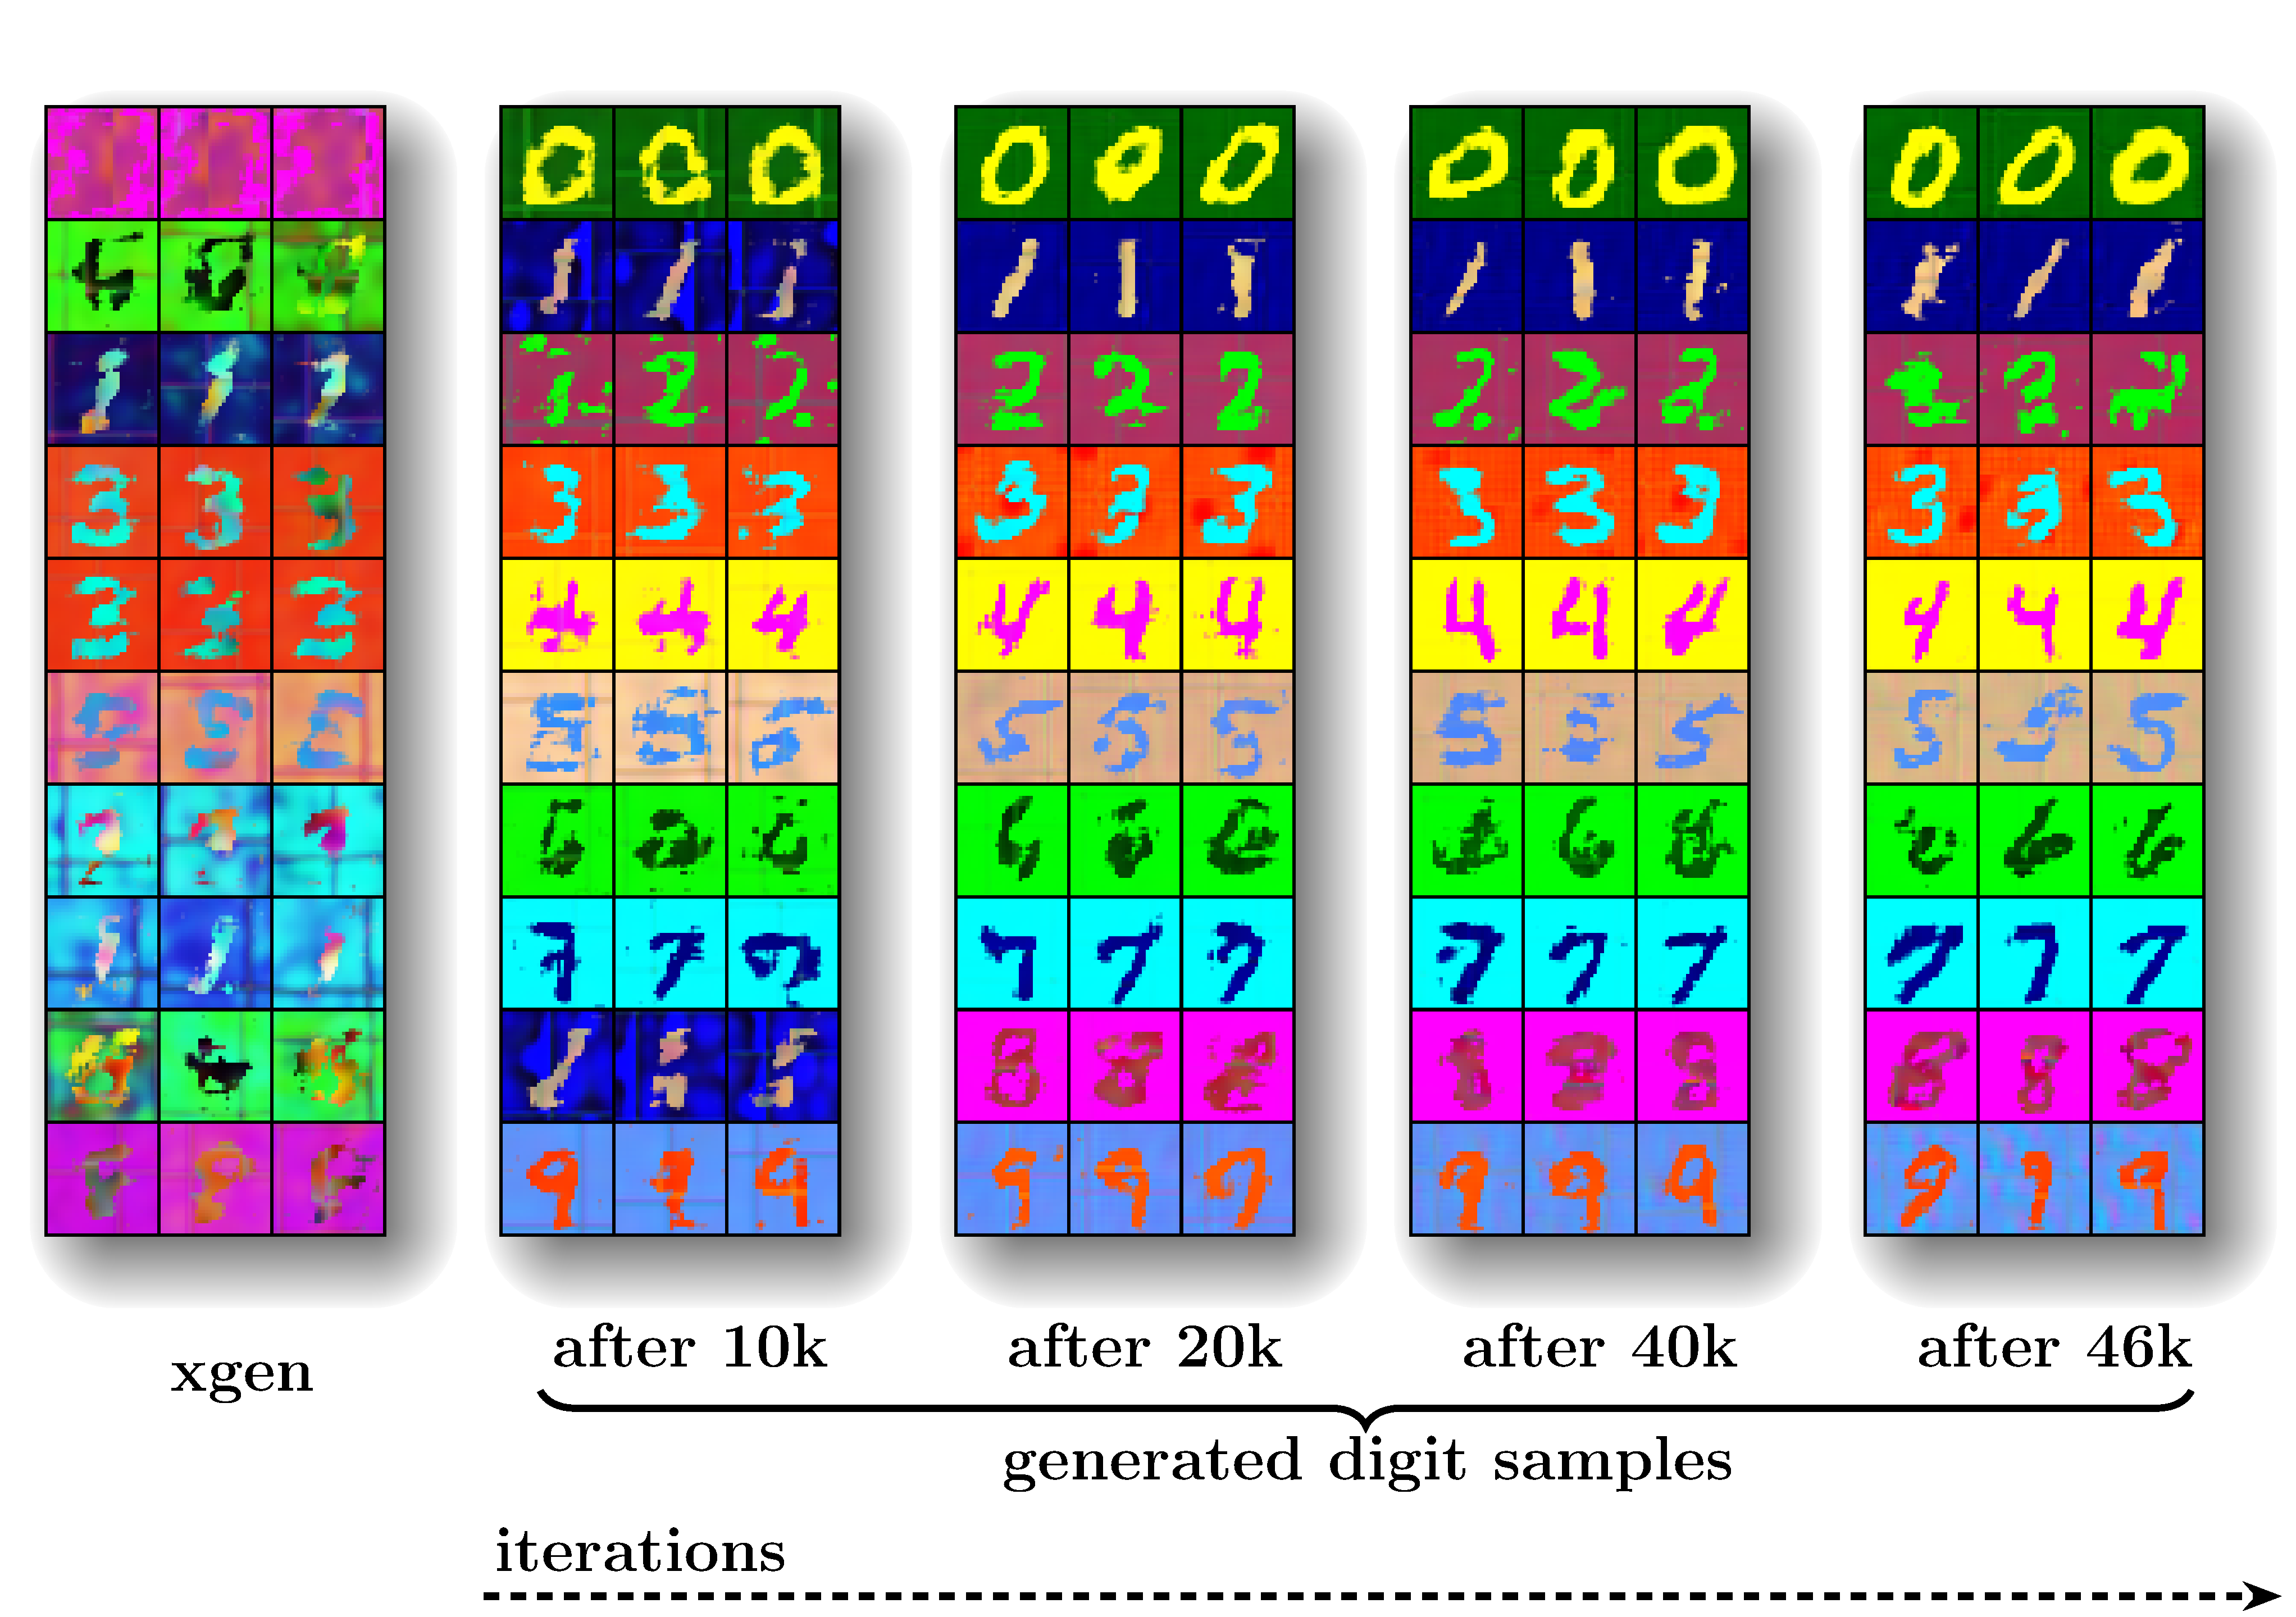
\includegraphics[width=0.8\textwidth,height=0.5\textwidth]{../openreview/images/x_gen_original.pdf}
    \caption{Double Colored MNIST samples obtained using default hyper-parameters mentioned in CGN \cite{sauer2021counterfactual}.
    }
    \label{fig:original_grid}
\end{figure}

\begin{figure}[ht!]
\centering 
    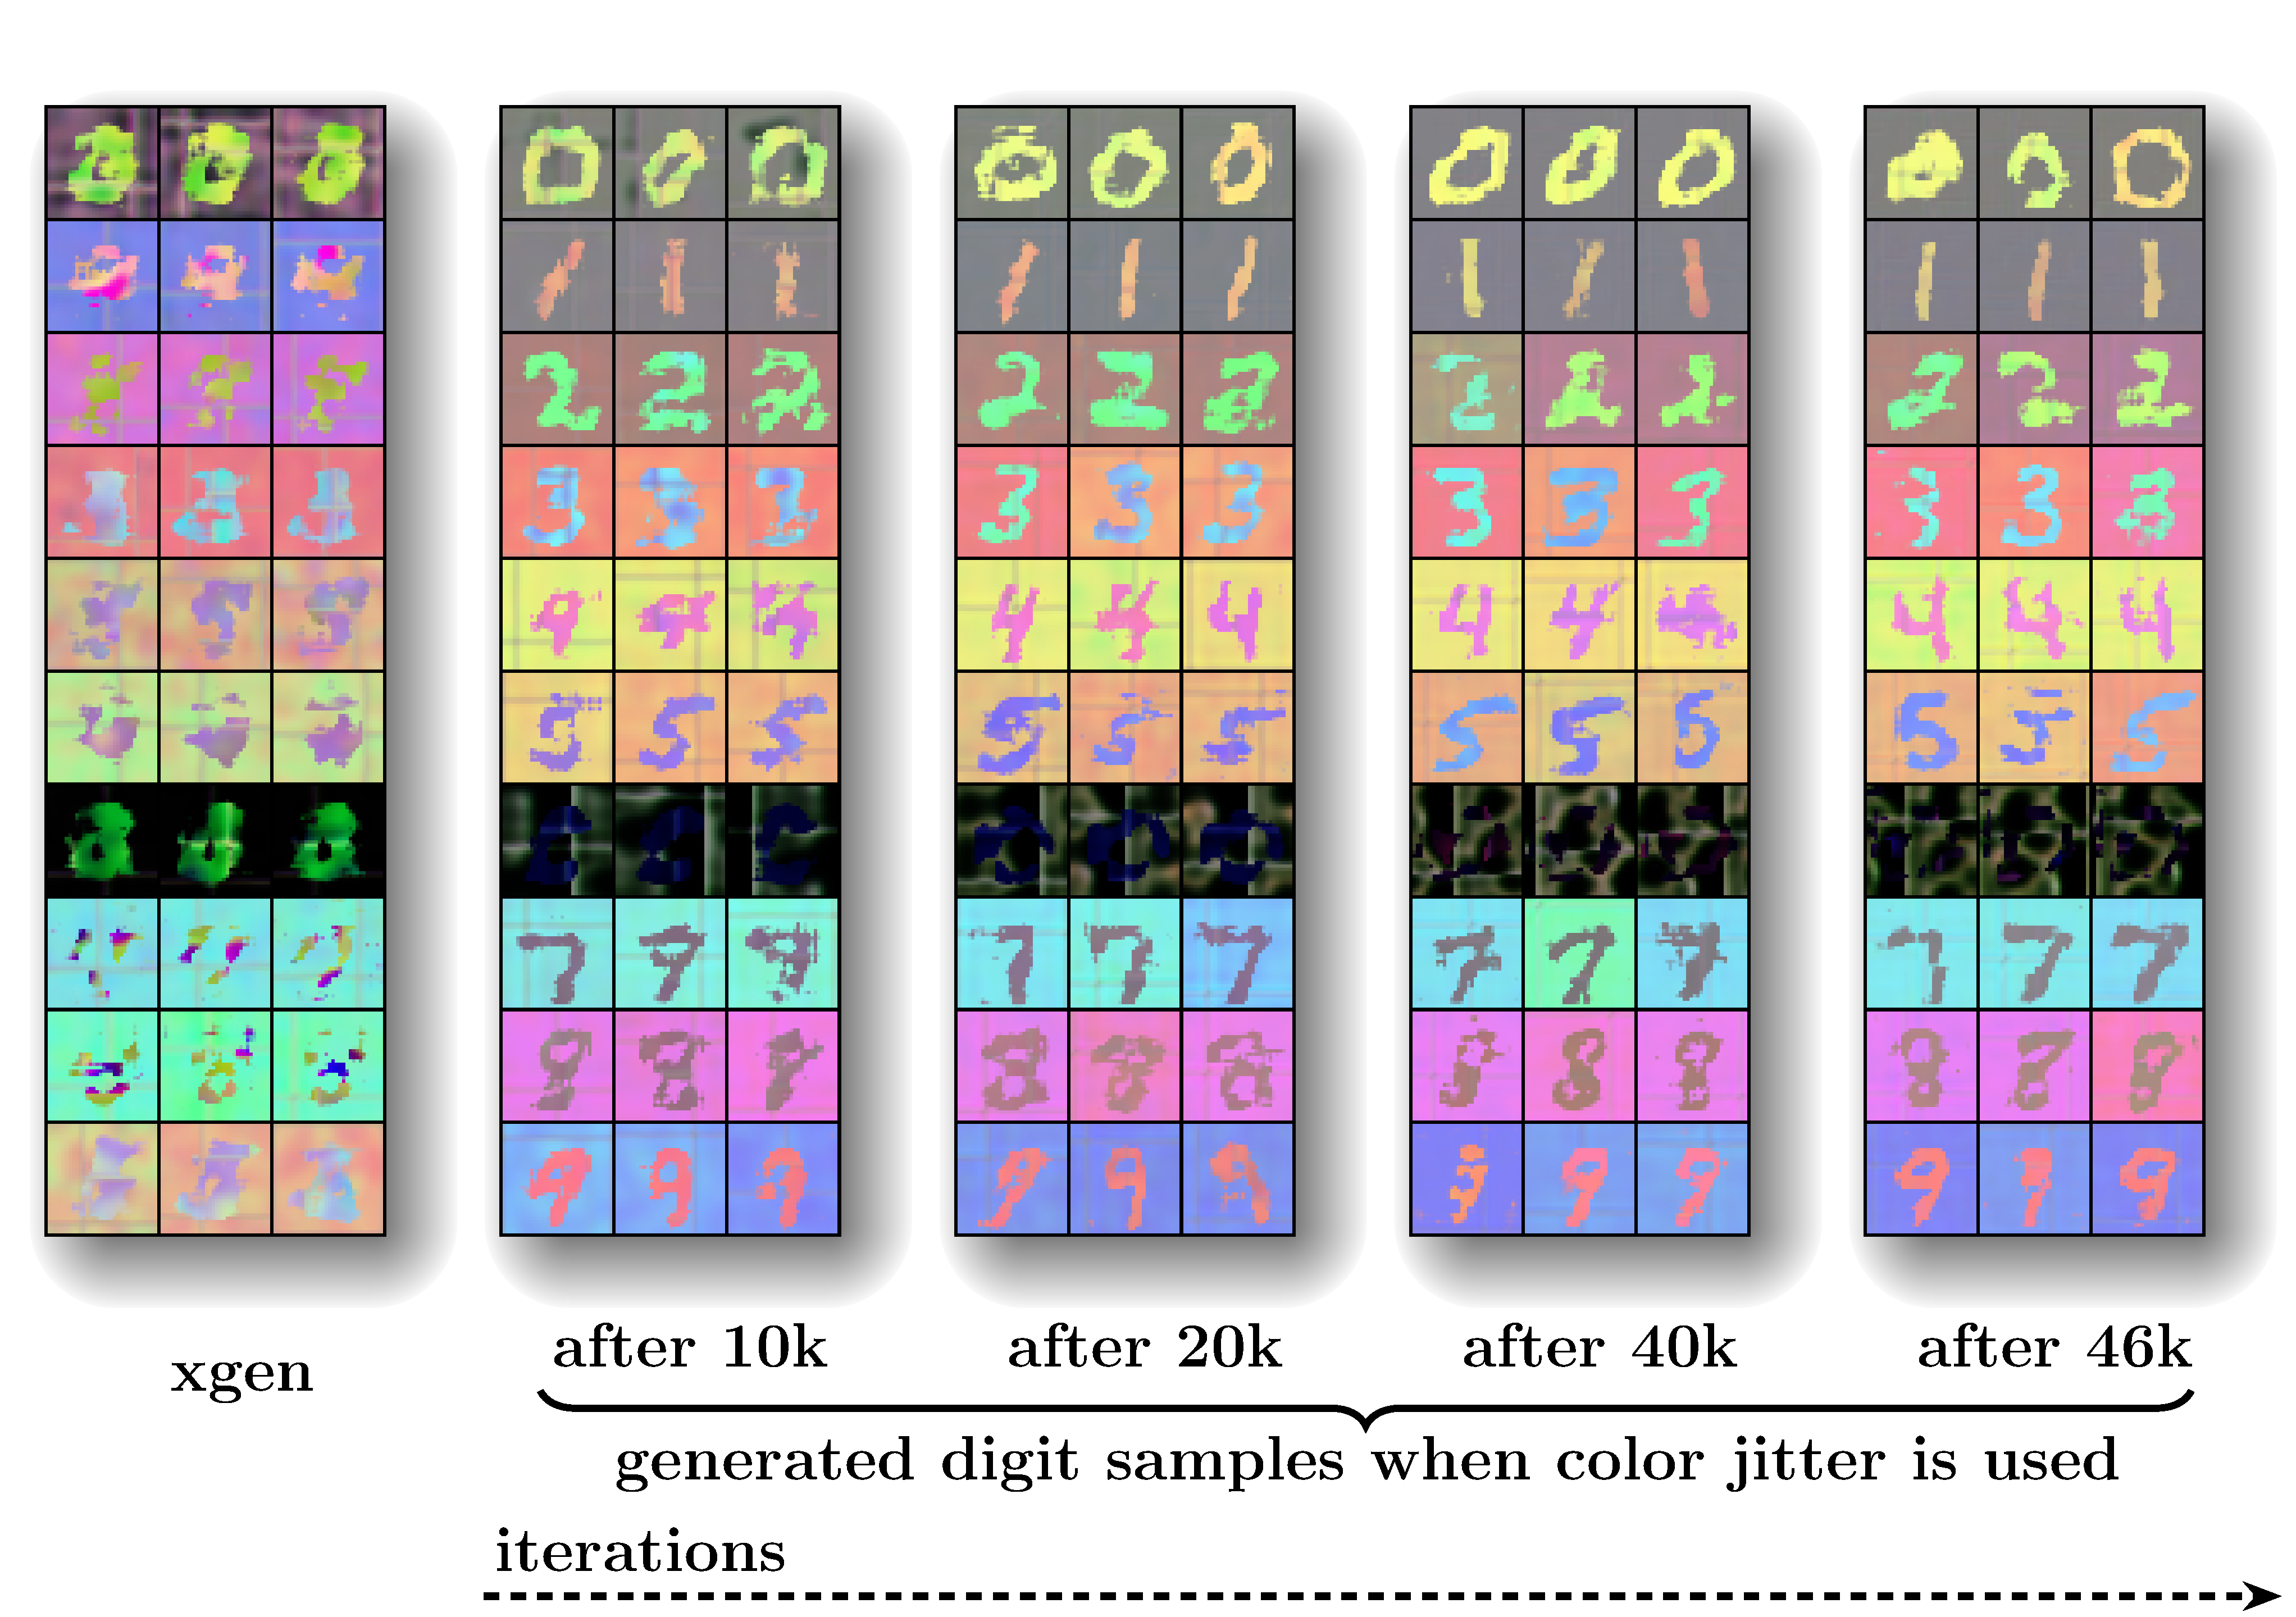
\includegraphics[width=0.8\textwidth,height=0.5\textwidth]{images/x_gen_data_augment.pdf}
    \caption{Double Colored MNIST samples obtained using addition of color jitter. We observe that it leads to generation of samples that are not indicative of the actual samples from the Double Colored MNIST dataset.  We observe that there is difference between with/without augmentation in terms of the brightness, contrast, overall image representations. Specifically, digit 6 loses its shape, texture, colors. Similarly, digits 0,1 are generated using different colors in contrast to Fig. \ref{fig:original_grid}. Therefore, the visual samples indicate possibly why the classifier's accuracy drops by around 10\%. 
    }
    \label{fig:data_augment_grid}
\end{figure}



